\documentclass[a4paper, uplatex]{jsarticle}

% 数式
\usepackage{amsmath,amsfonts}
\usepackage{bm}
% 画像
\usepackage[dvipdfmx]{graphicx}
\usepackage{tikz}
\usepackage{pgfplots}
\pgfplotsset{compat=newest}

\usepackage[deluxe]{otf}

% 表
\usepackage{booktabs}

\newcommand{\enumref}[1]{(\roman{#1})}

\begin{document}

\title{力学}
\author{}
\date{}
\maketitle

\tableofcontents
\newpage

\section{1次元運動}
\subsection{位置と座標}

物体の位置を表すために図\ref{fig:position}のような\textbf{座標}を用いる。

\begin{figure}[htbp]
  \centering
    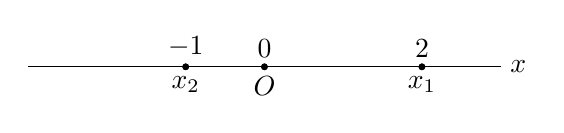
\begin{tikzpicture}
    % 一次元の座標軸
    \draw[-] (-3,0) -- (3,0) node[right] {$x$};

    % 原点O
    \filldraw[black] (0,0) circle (1pt) node[anchor=north] {$O$};
    \filldraw[black] (0,0) circle (1pt) node[anchor=south] {$0$};

    % 点x_1とx_2
    \filldraw[black] (2,0) circle (1pt) node[anchor=north] {$x_1$};
    \filldraw[black] (-1,0) circle (1pt) node[anchor=north] {$x_2$};
    \filldraw[black] (2,0) circle (1pt) node[anchor=south] {$2$};
    \filldraw[black] (-1,0) circle (1pt) node[anchor=south] {$-1$};
    \end{tikzpicture}
\caption{座標}\label{fig:position}
\end{figure}

基準となる位置を\textbf{原点}といい、記号\(O\)で表す。
次に、基準となる方向を決める。この方向に沿って原点から物体の位置まで移動した距離\(x\)によって位置を表す。
この\(x\)を物体の\(x\)座標という。例えば、図\ref{fig:position}では、右向きを正としている。

原点を変えると座標の値は変わる。例えば、図\ref{fig:position-move}では、原点\(O'\)を\(0.5\)にとった。
この結果、座標の値は0.5だけ増加する。これを、座標は座標系に相対的であるという。しかし、物体の位置は変わらない。
すなわち、ある位置に物体が存在するという事実がまずあり、それを人間が表す手段として座標がある。原点と基準になる方向を約束したものを\textbf{座標系}という。

\begin{figure}[htbp]
  \centering
    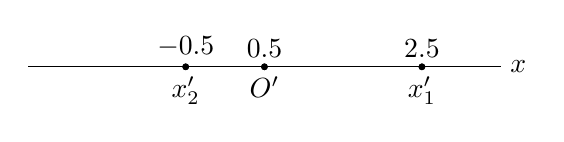
\begin{tikzpicture}
    \draw[-] (-2.5,0) -- (3.5,0) node[right] {$x$};

    % 原点O
    \filldraw[black] (0.5,0) circle (1pt) node[anchor=north] {$O'$};
    \filldraw[black] (0.5,0) circle (1pt) node[anchor=south] {$0.5$};

    % 点x_1とx_2
    \filldraw[black] (2.5,0) circle (1pt) node[anchor=north] {$x_1'$};
    \filldraw[black] (-0.5,0) circle (1pt) node[anchor=north] {$x_2'$};
    \filldraw[black] (2.5,0) circle (1pt) node[anchor=south] {$2.5$};
    \filldraw[black] (-0.5,0) circle (1pt) node[anchor=south] {$-0.5$};
    \end{tikzpicture}
  \caption{原点を移動させた座標}\label{fig:position-move}
\end{figure}

一般に運動は、物体の空間の位置、すなわち3つの座標によって考えるが、ここでは、1方向の運動に限って考える。
これを、\textbf{1次元運動}という。

物体が表\ref{tab:1d-motion}のように運動したとする。これをグラフに表すと図\ref{fig:1d-motion}のようになる。
このように、グラフに表すことで、直接物体を見なくても運動の様子がわかる。

\begin{table}[htbp]
  \centering
  \caption{1次元運動の例}\label{tab:1d-motion}
  \begin{tabular}{ccccccc}
  \toprule
  t & 0    & 1    & 2    & 3     & 4     & 5     \\
  x & 3.00 & 4.54 & 7.67 & 11.80 & 16.15 & 19.75 \\ \bottomrule
  \end{tabular}
\end{table}

\begin{figure}[htbp]
\centering
\begin{tikzpicture}
  \begin{axis}[
    xlabel={\( t \)},
    ylabel={\( x \)},
    xmin=0, xmax=5.2,
    ymin=0, ymax=22,
    xtick={0,1,2,3,4,5},
    ytick={10,20},
    grid=none,
    axis x line=bottom,
    axis y line=left,
  ]
\addplot[only marks, mark=*, mark options={fill=black}]
coordinates {(0,3.00) (1,4.54) (2,7.67) (3,11.80) (4,16.15) (5,19.75)};
\end{axis}
\end{tikzpicture}
\caption{1次元運動の例}\label{fig:1d-motion}
\end{figure}

各時刻ごとに物体はどこかの位置にある。すなわち、時刻を指定すれば座標の値が求まる。これは数学的には、座標\(x\)が時刻\(t\)の関数であると表される。
よって、数学的には\(x=f(t)\)と表されるが、物理では関数量がたくさん登場するので、関数記号と変数に同じ文字を使って
\begin{equation}
  x = x(t)
  \label{eq:1d-function}
\end{equation}
と書くことにする。

\subsection{速度}

物体の移動距離を経過時間で割った量を\textbf{速度}という。速度の単位はm/sである。

移動距離は座標の差で表される。時刻\(t_1\)に\(x_1=x(t_1)\)にいた物体が、時刻\(t_2\)に\(x_2=x(t_2)\)に移ったとする。このとき移動距離は\(d_{12}=x_2-x_1\)で表される。
\(d_{12}\)を\textbf{変位}という。
このときの速度は、経過時間が\(t_2-t_1\)であるから、
\begin{equation}
  v_{12} = \frac{d_{12}}{t_2-t_1} = \frac{x_2-x_1}{t_2-t_1} = \frac{x(t_2)-x(t_1)}{t_2-t_1}
  \label{eq:1d-motion}
\end{equation}
となる。例えば、図\ref{fig:1d-motion}の例では、\(v_{12}=(7.67 - 4.54)/(2 - 1)=3.13\mathrm{m/s}\)となる。
ところで、もし\(x_2<x_1\)ならば、\(d_{12}<0\)、したがって\(v_{12}<0\)となる。すなわち、座標を約束した方向と逆向きに移動するときには、
変位、速度は負と定義する。移動距離は変位の絶対値に当たり、速度の絶対値に当たる量を速さという。

図\ref{fig:1d-motion}の例の速度のグラフを図\ref{fig:1d-velocity}に示す。

\begin{figure}[htbp]
\centering
\begin{tikzpicture}
  \begin{axis}[
    xlabel={\( t \)},
    ylabel={\( v \)},
    xmin=0, xmax=5.2,
    ymin=0, ymax=22,
    xtick={0,1,2,3,4,5},
    ytick={10,20},
    grid=none,
    axis x line=bottom,
    axis y line=left,
  ]
\addplot[only marks, mark=*, mark options={fill=black}]
coordinates {(0.5,1.54) (1.5,3.13) (2.5,4.13) (3.5,4.35) (4.5,3.60)};
\end{axis}
\end{tikzpicture}
\caption{速度の例 (図\ref{fig:1d-motion}の\(x\))}\label{fig:1d-velocity}
\end{figure}

このように、物体の速度は一定とは限らないため、瞬間の速度を考える必要がある。
それには経過時間を短くすればよい、式\ref{eq:1d-motion}より、\(v_{12}\)は点1と点2を結ぶ直線の勾配であることがわかる。
点2を点1に近づけていけば、時刻\(t_1\)での速度は関数\(x(t)\)の点1での接線の勾配となることがわかる。数学では、これは微分で表される。すなわち、
\begin{equation}
  v(t_1) = \lim_{t_2 \to t_1} \frac{x(t_2) - x(t_1)}{t_2 - t_1} = \lim_{\Delta t \to 0} \frac{\Delta x}{\Delta t} = \frac{dx}{dt}
  \label{eq:1d-velocity}
\end{equation}
が成り立つ。

時刻\(t_1\)を変えていけば、一般の時刻\(t\)における速度が求められる。すなわち、速度もまた時間の関数であり、\(v = v(t)\)と表される。

以上より、\(x(t)\)と\(v(t)\)の関係は、
\begin{equation}
  \frac{dx}{dt} = \dot{x} = v(t)
  \label{eq:1d-v-x}
\end{equation}
と表される。

原点の位置を変えても、それが固定されていれば、変位は同じであるから速度は変わらない。しかし、原点自身が移動しているような座標系に移れば、速度の値も当然変化する。
この意味で、速度の値もまた一般には座標系に相対的である。

\subsection{加速度}

速度が一定ではなく、変化するとき、速度の時間変化率を考え、これを\textbf{加速度}という。加速度の単位はm/s\(^2\)である。

加速度の値は、\(v(t)\)図の勾配に当たる. 時刻\(t_0\)から\(t_1\)の間の加速度\(a_{01}\)は、
\begin{equation}
  a_{01} = \frac{v(t_1) - v(t_0)}{t_1 - t_0} = \frac{v(t_1) - v(t_0)}{t_1 - t_0}
  \label{eq:1d-acceleration}
\end{equation}
である. たとえば、図\ref{fig:1d-velocity}の、時刻\(t_{01}\)から\(t_{12}\)までの間の加速度は、
\(a_{012} = (3.13 - 1.54)/1 = 1.59\mathrm{m/s^2}\)となる。

速度の勾配が一定でない場合には、各瞬間ごとの加速度を考える。それには、\(x(t)\)の導関数として瞬間の速度\(v(t)\)を定義するのと同じように、
\(v(t)\)の導関数として加速度\(a(t)\)を定義すれば良い。すなわち、
\begin{equation}
  a(t) = \lim_{\Delta t \to 0} \frac{v(t + \Delta t) - v(t)}{\Delta t} = \lim_{\Delta t \to 0} \frac{\Delta v}{\Delta t} = \frac{dv}{dt}
  \label{eq:1d-acceleration-function}
\end{equation}
である。\(v=\dot{x}=dx/dt\)であるから、\(a(t)\)と\(x(t)\)の関係は、
\begin{equation}
  a(t) = \frac{dv}{dt} = \frac{d^2x}{dt^2} = \ddot{x}
  \label{eq:1d-a-x}
\end{equation}
となる。すなわち、\(a(t)\)は\(x(t)\)の\(t\)に関する2次導関数であって、これを点を二つつけた記号\(\ddot{x}\)で表す。

原点の移動速度が一定の座標系に移っても、すべての速度がその分変化するため加速度の値は変わらない。しかし、原点の移動速度が変化しているような座標系に移れば、加速度の値も当然変化する。
このように、加速度の値もまた一般には座標系に相対的である。

\subsection{位置の予測}
物体の位置の関数\(x(t)\)を\(t=0\)付近でテイラー展開すると、
\begin{equation}
  x(t) = x(0) + x(0)'t + \frac{1}{2}x(t)''t^2 + \frac{1}{3!}x(t)^{(3)}t^3 + \cdots
  \label{eq:1d-taylor}
\end{equation}
となる。また、速度と加速度の関係式 (\ref{eq:1d-v-x}) と (\ref{eq:1d-a-x}) より、
\begin{equation}
  x(t) = x(0) + v(0)t + \frac{1}{2}a(0)t^2 + \frac{1}{3!}x(t)^{(3)}t^3 + \cdots
  \label{eq:1d-taylor-2}
\end{equation}
と書ける。このように、ある時刻における速度、加速度、さらに高次の微分の情報が得られるにつれて、より正確な位置の予測ができる。

\subsection{慣性運動}
物体に対して、以下の2つの法則が成り立つ。

\begin{enumerate}
  \item 静止または等速度運動している物体は、外からの作用がなければ、その運動を続ける。 \label{enum:1d-inertia}
  \item 物体に外から力を作用させると、その速度が変化する。 \label{enum:1d-force}
\end{enumerate}

\ref{enum:1d-inertia}は、力がはたらかないときの運動、いわば自然な運動が、静止または速度一定の運動であるといってよい。この自然な運動を\textbf{慣性運動}といい、この法則を\textbf{慣性の法則}という。
静止は、速度が0の等速度運動であるため、その場合を含めて、「物体の慣性運動は等速度運動である」といい表せる。

\subsection{慣性座標系}
速度は座標系に相対的であるため、どのような座標系で運動を考えるのかという約束をしなければならない。

そこで、慣性の法則が成り立っているような座標系で運動の法則を議論することにする。このような座標系を\textbf{慣性座標系}という。
したがって、\ref{enum:1d-inertia}は、
\begin{quote}
  慣性座標系が存在し、そこで観測すれば、外からの作用を受けない物体は静止または等速度運動を続ける。
\end{quote}
ということになる。これを\textbf{ニュートンの第1法則}という。
\end{document}